\documentclass{article}
\usepackage{iclr2026_conference,times}
\usepackage[T1]{fontenc}
\usepackage{amsmath,amssymb,booktabs,graphicx,microtype}
\usepackage{hyperref}
\usepackage{placeins}
\usepackage{pdfpages}
\usepackage{listings}
\lstdefinestyle{pythonpseudocode}{
    language=Python,
    basicstyle=\footnotesize\ttfamily,
    keywordstyle=\bfseries,
    commentstyle=\itshape,
    showstringspaces=false,
    keepspaces=true,
    columns=fullflexible,
    breaklines=true,
    breakatwhitespace=true,
    frame=single,
    captionpos=b
}
\hypersetup{colorlinks=true,linkcolor=blue,urlcolor=blue,citecolor=blue}
\graphicspath{{figures/}}
\newcommand{\pending}[1]{\par\noindent\textbf{Pending:} #1\par}
\title{Homework 1:\\Backpropagation and Neural Networks}
\author{\textbf{[Zhang Zeyu]}\\Student ID: \textbf{[2026213422]}\\Deep Learning (84100343-0)\\Tsinghua University, Autumn 2026}
\iclrfinalcopy
\begin{document}
\maketitle
\lhead{Deep Learning (Autumn 2026) --- Homework 1}
\begin{abstract}
This coursework report includes the author's handwritten backpropagation solutions, the completed NumPy expert module, and a controlled comparison of dense and sparse mixture-of-experts language models.
\end{abstract}
\section{Part One: Backpropagation}
\label{sec:part1}
\pending{Insert the author's independent handwritten solutions as photographs or scans. No handwritten derivations have been generated for this draft.}
\begin{enumerate}
\item Forward computation for the numerical example: handwritten answer pending.
\item Softmax Jacobian and cross-entropy gradient: handwritten answer pending.
\item Parameter and shared-input gradients: handwritten answer pending.
\item Convolutional backpropagation and SGD: handwritten answer pending.
\end{enumerate}
% Put scans in figures/ and insert them here with \includegraphics.


\section{Part Two: Implementing the Experts}
\subsection{Task 1: Forward and backward implementation}
The NumPy module implements the expert MLPs, selected-expert gates, residual addition, and prediction head specified in the handout~\citep{handout}. Samples are stored in rows, while weight arrays retain the prescribed column-vector convention. Expert computations are batched using \texttt{einsum}. Unselected router logits are masked before Softmax, and the supplied mask is retained during finite-difference checks. Prediction log-probabilities are computed using a shifted log-sum-exp expression for numerical stability.

Backpropagation uses NumPy only, with no automatic differentiation. The mean-loss scaling is applied once at the prediction logits. The input gradient accumulates the expert, router, and direct residual paths; the ReLU derivative at zero is set to zero. The two-expert numerical case gives loss $1.0986122886681098$, and the supplied three-expert Top-2 case gives loss $1.184281870559786$.

\subsection{Task 2: Central-difference verification}
The official checker uses float64, perturbation $\epsilon=10^{-6}$, and a fixed selection mask away from routing ties and ReLU kinks. Table~\ref{tab:numpy-gradients} reports the maximum normalized error for every parameter family and the input, using the normalization in the handout. All errors are below the required $10^{-5}$ threshold.
\begin{table}[ht]
\centering
\small
\caption{Maximum normalized central-difference errors.}
\label{tab:numpy-gradients}
\begin{tabular}{lrr}
\toprule
Quantity & Two-expert example & Three-expert Top-2 \\
\midrule
$W_1$ & 1.404e-11 & 1.370e-10 \\
$b_1$ & 1.075e-10 & 1.234e-10 \\
$W_2$ & 4.084e-11 & 1.173e-10 \\
$b_2$ & 9.348e-11 & 1.000e-10 \\
$G$ & 6.077e-11 & 8.208e-11 \\
$C$ & 4.270e-11 & 1.137e-10 \\
$b_c$ & 6.443e-11 & 1.600e-10 \\
$x$ & 4.142e-11 & 1.083e-10 \\
\bottomrule
\end{tabular}
\end{table}


The supplied faulty variant explicitly subtracts the direct residual contribution from the otherwise complete input gradient. It therefore omits the identity path from the input to the residual sum. Its normalized input error rises to $0.133333$ in the two-expert case and $0.279717$ in the sparse case. This distinguishes an incorrect shared-input gradient from the parameter gradients, which can still be correct when an input path is omitted.

\subsection{Task 3: Fixed-batch training}
Training uses the supplied 128 examples and initialization, fixed context features, 400 full-batch SGD updates, and learning rate $0.2$. No hyperparameter search was performed. Training cross-entropy decreases from $5.593877$ to $1.870696$ (Figure~\ref{fig:numpy-loss}). Table~\ref{tab:numpy-predictions} shows the three examples selected by the provided runner. Two are incorrect despite the loss reduction; this is a training demonstration, not evidence of generalization.
\begin{figure}[ht]
\centering
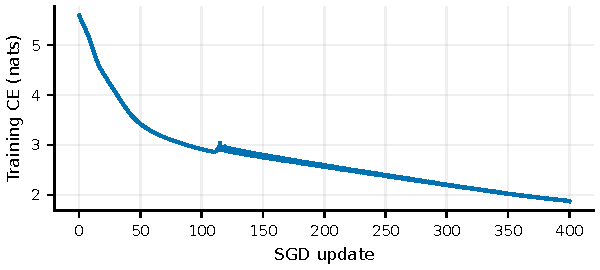
\includegraphics[width=.72\linewidth]{numpy_loss.pdf}
\caption{Mean training cross-entropy for the provided NumPy batch. The curve includes the initial loss and the loss after each of 400 SGD updates.}
\label{fig:numpy-loss}
\end{figure}
\begin{table}[ht]
\centering
\small
\caption{Three predictions after 400 NumPy SGD updates. Parentheses contain byte values.}
\label{tab:numpy-predictions}
\begin{tabular}{lll}
\toprule
Four-byte context & Target & Prediction \\
\midrule
\texttt{tle'} & s (115) & space (32) \\
\texttt{est=} & a (97) & e (101) \\
\texttt{u\textvisiblespace{}as} & space (32) & space (32) \\
\bottomrule
\end{tabular}
\end{table}

\FloatBarrier


\section{Part Three: A Small MoE Language Model}
\subsection{Task 1: Implementation, training, and evaluation}
Each expert applies a $64\rightarrow128\rightarrow64$ MLP with ReLU. The router selects the two largest logits from 16 experts and normalizes their weights over the selected set. Separately, probabilities over all experts feed the provided load-balancing objective. Dispatch gathers only the selected rows for each expert, evaluates those rows, multiplies by the corresponding gates, and accumulates results into the output. No expert is evaluated on all tokens followed by output masking.

The official CPU diagnostic executes exactly 14 selected token--expert pairs for seven tokens with $k=2$, compared with 21 pairs for dense execution. Its maximum output error is zero and its maximum gradient error is $1.11\times10^{-16}$ against the dense reference. Paired routing records are preserved at each position. Both normal routing and position-wise route perturbation pass prefix invariance, with maximum prefix-logit error zero. These checks establish the tested numerical and causal properties, rather than model quality.

\paragraph{Protocol.}
The supplied two-block causal context model uses dimension 64, four attention heads, sequence length 64, and a 256-byte vocabulary. The computation-matched dense FFN has hidden width 264; the parameter-matched FFN has width 2056. All runs use seed 416, 3000 updates, and batches of 32 sequences, with equal sampling from Shakespeare and Python. AdamW uses the supplied base learning rate $0.002$, weight decay $0.01$, cosine schedule with a 0.15 floor fraction, and gradient clipping at 1. The MoE load-balancing coefficient is $0.01$. Common non-FFN initialization and the sampling order are shared across configurations. Runs use PyTorch 2.8.0 on an arm64 CPU with four threads.

Validation is logged every 500 updates using 20 batches per domain; the checkpoint with the lowest validation CE is selected. In all three runs that checkpoint is at update 3000. Figure~\ref{fig:language-curves} reports the recorded training and validation curves. Training points are individual current-batch losses, not epoch means; their increase at update 3000 does not imply an increase in validation loss. Held-out test evaluation uses nonoverlapping full-length packs within document boundaries: 111,488 text targets and 1,179,520 code targets. The main CE is the unweighted mean of the two domain CEs, and perplexity is its exponential. Test data are not used for checkpoint selection.

\begin{figure}[ht]
\centering
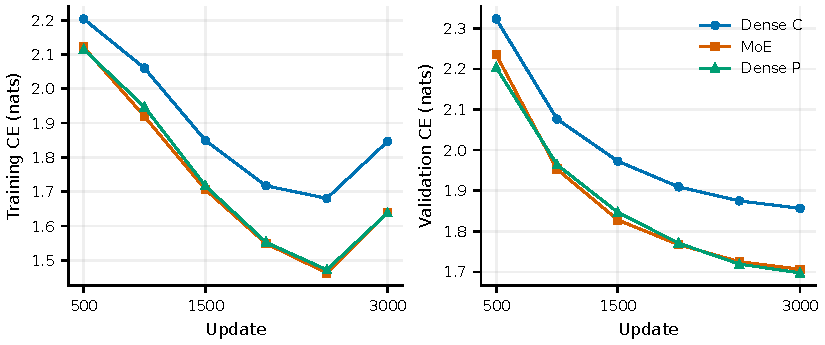
\includegraphics[width=\linewidth]{language_curves.pdf}
\caption{Training and validation cross-entropy for the three configurations under the same 3000-update protocol. Training values are sampled batches at logging steps; validation values average the fixed evaluation procedure. C and P denote computation-matched and parameter-matched dense models.}
\label{fig:language-curves}
\end{figure}

\subsection{Task 2: Capacity, computation, routing, and usage}
Table~\ref{tab:language-results} reports domain metrics, total parameters, matrix MACs per token, and full-batch latency. MAC counts include attention projections and attention products, router, expert matrices, and prediction head across both blocks; they exclude non-matrix operations. With $D=64$, $T=64$, $E=16$, and $k=2$, the per-token count is
\begin{equation}
2\left[4D^2+2TD+F\right]+256D,\qquad
F=\begin{cases}2DH, & \text{dense},\\ ED+2kDH, & \text{MoE}.\end{cases}
\end{equation}
Latency includes dispatch and uses $B=32$, $T=64$, ten warmups, and the median of 30 no-gradient forward passes on the same CPU.
\begin{table}[ht]
\centering
\small
\caption{Test results and costs. C/P denote computation/parameter matching; latency is in milliseconds per full batch.}
\label{tab:language-results}
\begin{tabular}{@{}lrrrrrrr@{}}
\toprule
Model & Params & MACs/token & Text CE & Code CE & Mean CE & PPL & ms \\
\midrule
Dense C & 139,024 & 133,120 & 1.9732 & 1.7985 & 1.8858 & 6.5919 & 2.458 \\
MoE & 603,264 & 133,120 & 1.8969 & 1.6289 & 1.7629 & 5.8292 & 5.107 \\
Dense P & 601,360 & 591,872 & 1.9068 & 1.6255 & 1.7661 & 5.8482 & 8.083 \\
\bottomrule
\end{tabular}
\end{table}


\paragraph{Capacity and quality.}
At the same 133,120 matrix MACs per token, MoE stores 4.34 times as many parameters as the computation-matched dense model and reduces test CE by 0.1230 nats in this run. Against the parameter-matched dense model, whose parameter count differs by only 0.316\%, MoE has similar test CE (difference $-0.0032$ nats), using about 22.49\% of its matrix MACs. This small quality difference from one training seed is not evidence of a reliable advantage.

\paragraph{Measured latency.}
MoE takes 5.107 ms per batch, compared with 2.458 ms for computation-matched dense and 8.083 ms for parameter-matched dense. Thus equal MACs do not imply equal latency: sparse execution entails gather/scatter, dispatch, and many smaller matrix operations. The measurement is consistent with those overheads but does not isolate their individual costs. The comparison fixes updates and sampling order, rather than wall-clock budget or convergence.

\paragraph{Routing control.}
The supplied diagnostic exchanges paired expert IDs and gate weights across sequences at the same position in the last layer. It changes neither time positions nor expert--token counts. The trained checkpoint passes prefix invariance for both routing modes, with error zero. The three routing seeds 20261004, 20261005, and 20261006 produce diagnostic CEs of 2.958319, 2.960190, and 2.957595, respectively. Their mean is 2.958701, compared with normal CE 1.762883, an increase of 1.195818. These results indicate sensitivity to the original paired route assignments at this checkpoint. Because predictions depend on other sequences in the batch and the intervention changes both expert IDs and weights, this diagnostic is neither standalone language-model performance nor a causal estimate of the training benefit of routing.

\begin{figure}[p]
\centering
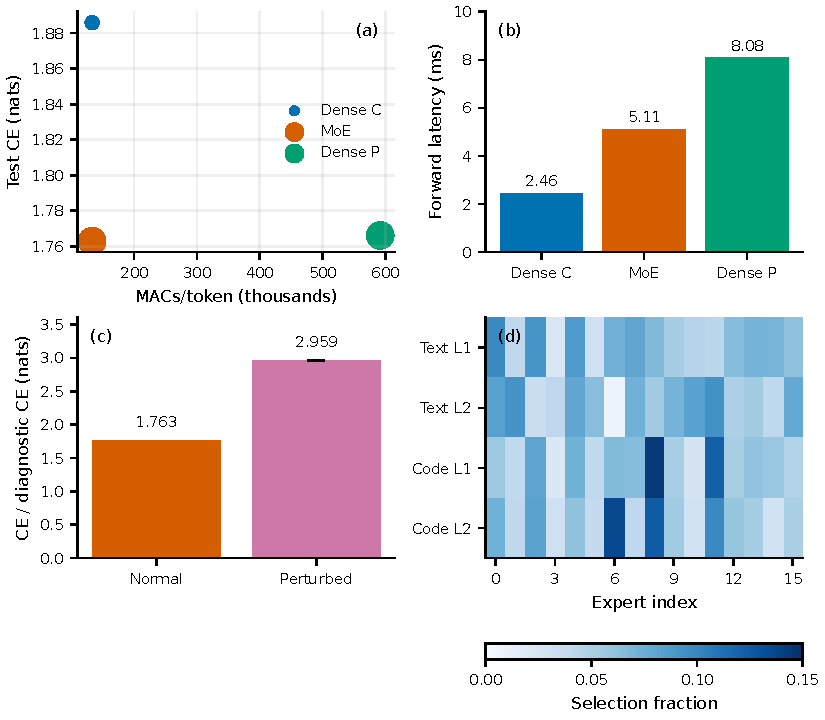
\includegraphics[width=\linewidth]{task2_analysis.pdf}
\caption{Task 2 comparison. (a) Test quality versus matrix cost; marker area encodes total parameters. (b) Full-batch forward latency including dispatch. (c) Normal CE and the batch-dependent route-perturbation diagnostic; error bars span the three fixed routing seeds, not independent training runs. (d) Expert selection fractions, normalized within each domain and layer. Expert indices are zero-based.}
\label{fig:routing}
\end{figure}

\paragraph{Expert usage and limitations.}
Figure~\ref{fig:routing} shows domain-dependent routing frequencies. For example, in the second layer, expert 6 receives about 0.87\% of text assignments but 13.59\% of code assignments. These frequencies establish different usage patterns, not semantic specialization or an interpretation of what that expert computes. The experiment uses a single model seed, a small fixed corpus, and CPU timing; variation across training seeds and hardware is not measured. The perturbation preserves routing counts but does not preserve each token's assigned experts or gates.

\subsection{Task 3: Independent investigation}
\pending{Define the author's testable question, control, experiments, interpretation, and limitation. No new investigation has been performed for this draft. The completed Task 2 diagnostic should not be relabeled as an independent investigation.}
\FloatBarrier


\FloatBarrier
\section*{Reproducibility and completion status}
The results follow the provided course handout~\citep{handout}. Run the following commands from the release directory, using an environment with the supplied requirements:
\begin{verbatim}
python NumPy/run.py --check --train
python MoE/diagnostics.py --check
python MoE/train.py --mode all --device cpu
python MoE/diagnostics.py --device cpu
python MoE/gate_ablation.py --device cpu
\end{verbatim}
The bundled data snapshots contain the NumPy results (\path{data/numpy.json}), language-model results (\path{data/language.json}), and source hashes (\path{data/run_provenance.json}). Run \path{prepare_results.py} to rebuild the tables and vector figures. The original logs and selected MoE checkpoint remain in the release's \path{results/} directory. NumPy results were rerun on the current implementation when preparing this report and reproduce the previously checked values.



\section*{AI Use Statement (draft for author review)}
OpenAI Codex assisted with reviewing the NumPy and PyTorch implementations, diagnosing errors, and improving variable names, comments, and input checks in the NumPy module.
Codex also ran the supplied checks and experiments, generated result figures and tables, and prepared this LaTeX draft using the ICLR template.
The reported measurements were verified against saved execution logs and official diagnostics; no Part One handwritten derivations or Part Three independent-investigation results were generated.
The assistance included edits to core NumPy code, so this statement does not assert that all assistance falls within the course's restriction to syntax and environment help for core programming tasks.
The author must review the assistance against the course rules and personally confirm responsibility for the final submission.

\end{document}
